\documentclass[a4paper,10pt,hidelinks]{scrartcl}

% packages
\usepackage[english]{babel}
\usepackage{graphicx}
\usepackage{hyperref}
\usepackage{url}
\usepackage{fontspec}
    \setmainfont{Arial}
    \setsansfont{Arial}
    \setmonofont{Fira Code}
\usepackage{fancyhdr}
\usepackage[paper=a4paper,left=20mm,right=20mm,top=40mm,bottom=25mm,headheight=40mm]{geometry}
\usepackage{tabto}
\usepackage{sectsty}
\usepackage{afterpage}
\usepackage{listings}
\usepackage{blindtext}
\usepackage{float}
\usepackage{wrapfig}

\hypersetup{
    colorlinks=true,
    linkcolor=black,
    filecolor=blue,      
    urlcolor=blue,
}

% global options
\renewcommand{\baselinestretch}{1.25}

\lstset{basicstyle=\small\ttfamily,captionpos=b,xleftmargin=0.25in,xrightmargin=0.25in}

% header/footer
\pagestyle{fancy}
\renewcommand{\headrulewidth}{0pt}
\renewcommand{\footrulewidth}{0pt}
\rhead{
\includegraphics[width=40mm]{pics/header-2.png}}
\rfoot{
\includegraphics[width=40mm]{pics/footer.png}}
\fancypagestyle{firstpage}{
    \rhead{
\includegraphics[width=40mm]{pics/header-1.png}}
}
\cfoot{}

\newcommand{\imgref}[1]{{figure \ref{#1} on page \pageref{#1}}}

\begin{document}

\section*{\fontsize{18}{20}\selectfont Object detection in fine-art photography}
\thispagestyle{firstpage}

\textbf{Themenbereiche:} \tabto{4cm} Artificial Intelligence, Visual Computing

\noindent
\textbf{Studierender:} \tabto{4cm} Fabian Meyer

\noindent
\textbf{Betreuungsperson:} \tabto{4cm} Dr. Simone Lionetti

\noindent
\textbf{Experte:} \tabto{4cm} Roman Bachmann, Swisscom

\noindent
\textbf{Keywords:} \tabto{4cm} Object detection, Machine learning, Computer vision, Photography

\section{\fontsize{14}{16}\selectfont Initial task}

Object detection is an important computer vision and machine learning task that consists in the localisation and classification of items within digital images. The business and industry applications of this technology are growing in number and relevance, especially because of the tremendous progress, largely driven by deep learning, that has been made in recent years.

The success of object detection models is usually measured with benchmark metrics on standard datasets such as MNIST, PASCAL VOC, ImageNet, COCO and Open Images. These reference scores summarise a complex set of performance parameters and are essential for a meaningful comparison of different approaches. Precisely because they are extremely synthetic, however, it is important to assess the quality of results with other, more ingenuous criteria.

\section{\fontsize{14}{16}\selectfont Results}

During the project cycle the following results have been achieved:

\begin{itemize}
	\item A dataset from different artists with different styles has been gathered
	\item Multiple object detection frameworks and models have been tested on these images of fine-art photography
	\item The most promising framework (mmdetection) and model (Mask R-CNN) have been selected
	\item A program that takes in an image and puts out a tidied up version with all objects found in it has been developed
	\item The program has been converted into a web app
	\item The web app has been deployed on the EnterpriseLab infrastructure
	\item %TODO retraining
\end{itemize}

\noindent
The web application can be viewed at: \url{http://bdaf20-iameyer.enterpriselab.ch}.

\noindent
In sum the performance of the Mask R-CNN model depends on the following criteria:

\begin{itemize}
	\item Class of objects in the image (included in COCO-dataset or not)
	\item Size of objects in the image
	\item Degree to which an object is visible and is shown in a natural style
	\item ...
\end{itemize}

\noindent
When applied to images of fine-art photography we can observe that performance is very variable because different photographers use different styles to depict their objects in their images. For example when using an image with a lot of smaller objects (like Andreas Gursky does), performance is rather poor compared to an image with less number and bigger objects. However with retraining %TODO retraining

\section{\fontsize{14}{16}\selectfont Solution concept}

\begin{wrapfigure}{r}{0.333\textwidth}
	\center{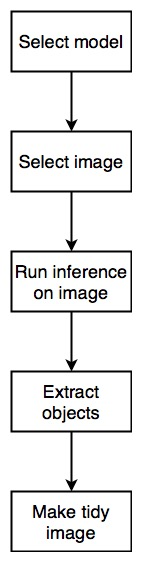
\includegraphics[width=75pt]
	{pics/control-flow.jpg}}
	\caption{\label{fig:control-flow} Control-flow diagram}
\end{wrapfigure}

The web application takes in images either from a selection (hosted on the server) or via upload or via a url. Then the model starts inference on the chosen image. The chosen model will detect potential objects in the image and returns them as a data structure, containing masks, bounding boxes, name of class and confidence score. \newline The program takes in the four results from the model and cuts out all objects from the original image. The found objects will be depicted on a new image in a grid-like fashion.

Cutting out the objects is possible with the bounding box and the object mask alone. One can cut out an object with the bounding box and colour all pixels for example with white colour which do not belong to the mask.

As nowadays most of research and work in the field of deep-learning is done in Python, Python has been chosen as the language to develop the full project. To transform the program into a full working web application, \href{https://dash.plotly.com}{Plotly Dash} has been chosen. Dash is using JavaScript technologies under the hood to get a Python app running on a web server.

For the framework, \href{https://github.com/open-mmlab/mmdetection/}{mmdetection} has been chosen because of its high level API and ease to use. As mmdetection (like most frameworks) needs a GPU for training and inference, \href{https://github.com/akarazniewicz/smd}{smd} (a wrapper around mmdetection models) has been chosen as a way to do inference on CPU.

%TODO smb

One can see a high-level view of the program in image: \imgref{fig:control-flow} and a sample output image in \imgref{fig:tidy-image}

\begin{figure}[!h]
	\center{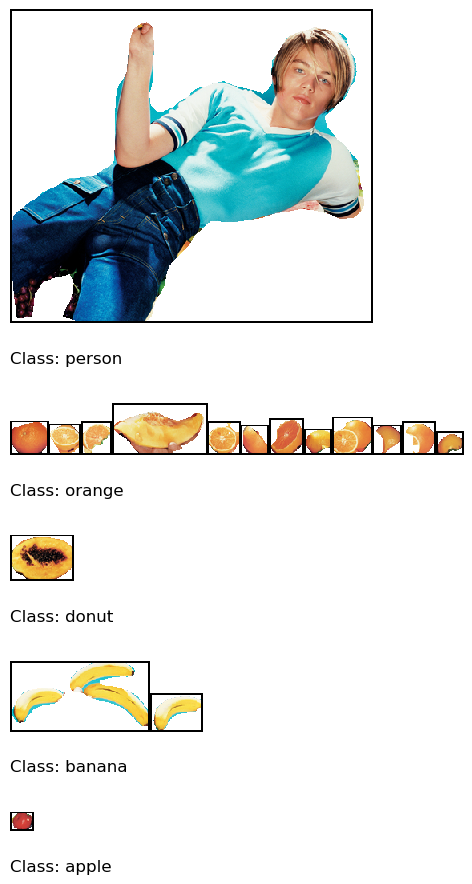
\includegraphics[width=250pt]
	{pics/tidy-image.jpg}}
	\caption{\label{fig:tidy-image} Sample output image}
\end{figure}

\section{\fontsize{14}{16}\selectfont Special challenges}

The biggest challenge was to get a model running on a standard CPU, for development purpose but also for deployment on a server. As most deep-learning networks are trained with GPUs, the easiest (and also most performant) way to deploy an app would be to use a GPU environment. However there are some frameworks that do accept GPU-trained networks and can use a CPU for inference. Still, using a CPU for inference results in much longer computation time.

\section{\fontsize{14}{16}\selectfont Outlook}

%TODO

In a further work, more models could be retrained to gain a deeper understanding of the detection of objects in images from different photographers. One could for example train a model on images from one photographer and test it on images from another photographer that contains the same classes of objects in it.

\end{document}
